\documentclass[12pt]{book}
\usepackage{graphicx}
\usepackage[a4paper,inner=36mm,outer=18mm,top=30mm,]{geometry}
%\usepackage[doublespacing]{setspace} 
\usepackage{bm}
\usepackage{siunitx}
\usepackage{titling}
\usepackage{hyphenat}
\usepackage{amsmath,amsfonts,amssymb,amsthm,mathtools}
\usepackage{hyperref}
\usepackage{bbm}
\usepackage{gensymb}
\usepackage{calc}
\usepackage{tabto}
\usepackage{natbib}

\DeclareMathOperator*{\argmin}{argmin}
\DeclareMathOperator*{\argmax}{argmax}

\begin{document}

\title{Thesis}
\author{Emilio Dorigatti}

\maketitle

\section*{Summary}
todo

\tableofcontents

\chapter{Introduction}

\section{Problem}

Climatology, or climate science, studies the long-term average weather conditions. In the last few decades, climate scientists found solid evidence of ongoing changes in Earth's climate, most notably, a general increase in average temperature; in the long run, this and other changes can potentially have a devastating impact on life on our planet. Regardless of the causal effect of human activities on it, having a solid understanding of the climate allows us to find the best way to mitigate its change, and possibly prevent it completely.

Climate science is an extremely difficult field, for a number of reasons. First, climate is evident, by definition, only over long periods of time and large distances, making the usual scientific approach of testing hypotheses by conducting experiments inapplicable; instead, climate scientists have to rely on historical data. Second, the atmosphere is a complex and chaotic system, which must be described through systems of nonlinear differential equation. They can be used to create numerical simulations, and the resulting predictions compared to historical data to assess the accuracy of the theory. Furthermore, the chaotic character of the atmosphere makes it impossible to study parts of it in isolation from others, as small scale phenomena affect large scale ones, and vice versa. In spite of this, it is useful to split the atmosphere in vertical layers and horizontal zones, in order to differentiate among conditions and phenomena typically occurring in one area or the other.

Usually, the troposphere is referred to as the lowest layer of the atmosphere, but it can actually be subdivided in more sub-layers, the lowest of which is the \emph{atmospheric boundary layer}: it is the region of the atmosphere that is affected by the conditions of the surface. Most human activities happen in this layer, and it is responsible for a large part of the diffusion and transport of aerosol such as, among others, pollutants. Yet, the physics governing the atmospheric boundary layer is not fully understood, and the theory is lacking. One important issues in the study of the atmospheric boundary layer is the derivation of flux-profile relationships for wind and temperature: they essentially relate the transport of momentum and heat by the wind (flux) with the change of wind speed/temperature with altitude (profile). The state of the art relationships are defined by the Monin-Obukhov Similarity theory in terms of the instability parameter $\xi$, computed as the height above surface scaled by turbulence due to horizontal wind and vertical air movement due to variations in heat. Difficulties in measurements of relevant quantities make this theory accurate only up to 10-20\%, and applicable in a restricted set of conditions.

In stark contrast to the traditional, top-down approach of science, recent developments in information technology made bottom-up approaches possible. In this new way of thinking, existing data is used to automatically infer the "best" explanation for the measurements at hand, the underlying laws that originated that data. The field that makes this possible is called Machine Learning: it takes advantage of several methods coming from statistics, information theory, optimization theory, etc., to make computers learn from examples. Together with Natural Language Processing and Automated Planning, it is one of the three main branches of Artificial Intelligence, the sub-field of Computer Science that studies ways of making machines behave intelligently.

todo more fluff about ml ?

\section{Research Question}
Currently, limitations of the validity of the Monin-Obukhov similarity theory are not believed to be a likely explanation for the high scatter that is found in experimental studies, unless in highly stable conditions \cite{basicatm}. With the availability of micro-meteorological data from specialized observation sites such as Cabauw, in the Netherlands, and the recent developments in Machine Learning, this conjecture can be finally put to the test. More specifically, we pose the following \\

\textbf{Research Question 1:} Is it possible to use the data from the Cesar database to improve the Monin-Obukhov model of the flux-profile relationships, by using more predictors besides the instability parameter? \\

\textbf{Research Question 2:} (in case of an affirmative answer to the first research question): What impact do the different features have on the quality of the prediction? \\

Affirmative answers to these question would contribute to improve the quality of current global circulation models (large scale climate simulations). \cite{sheba} shows that, at least in difficult conditions, several simulation models produce flux estimates that are highly inaccurate, presenting low correlation (mostly below 0.3) and errors that are as large as the fluxes themselves. Since errors in the simulation accumulate over time, even slight improvements can greatly improve the accuracy of the results after years of simulated time. Improved flux-profile relationship can, therefore, yield more accurate estimates of the fluxes.

\section{Research Methodology}
todo

\section{Ethics and Sustainability}

reproducibility: using open data, following standards of reproducible research (open source and jupyter notebooks)

\section{Outline}
todo

\chapter{Background}
This chapter introduces the basic concepts the reader should be qualitatively familiar with, in order to understand the content of this thesis. It is assumed readers are already knowledgeable of simple mathematical concepts, such as calculus, linear algebra, statistics, and probability theory. Readers acquainted with the material should feel free to skip this chapter.

\section{Fluid Dynamics}
Fluid dynamics is the discipline that studies the flow of fluids; it has several branches that study different fluids, such as aerodynamics (the study of air motion) and hydrodynamics (the study of water motion). These disciplines are routinely applied when designing cars, airplanes, ships, pipelines, etc.

\subsection{Laminar and Turbulent flow}
There are two distinct ways in which particles in a fluid can move: laminar flow and turbulent flow. In the former, all the particles move orderly, perhaps with a different speed, but all in the same direction, whereas in the latter the movement of particles is highly chaotic and unpredictable, and tends to dive rise to eddies of varying sizes. People are most familiar with the distinction between the two through the smoke rising from a cigarette, which starts smooth and becomes turbulent shortly thereafter, as in figure \ref{fig:smoke}. The kind of flow in under specific conditions can be predicted using the Reynolds number $Re$, which is the ratio between inertia forces, favoring turbulent flow, and viscosity forces, stabilizing the fluid towards laminar motion:

$$
Re=\frac{\rho u L}{\mu}=\frac{uL}{\nu}
$$

With $\rho$ the density of the fluid, $u$ its velocity, $L$ a characteristic linear dimension of the system under consideration, $\mu$ and $\nu$ the kinematic and dynamic viscosity of the fluid. The viscosity describes, intuitively, how much the molecules of the fluid tend to stick together and resist motion by generating drag. For example, water has low viscosity, and honey has high viscosity.

Since turbulence is random, it is usually studied in terms of the statistical properties of physical quantities through the Reynolds decomposition; given a quantity $a(s,t)$ which varies in space and time, we can compute its average

$$
\overline{a}(s)=\frac{1}{T}\int_{T_0}^{T_0+T}a(s,t)dt
$$

and the deviation from the average

$$
a'(s,t)=a(s,t)-\overline{a}(s)
$$

By definition, $\overline{a'}=0$, which means that all the effects of turbulence are contained in $a'$. Common statistical properties such as variance and covariance are expressed respectively as $\overline{a'a'}$ and $\overline{a'b'}$.

\begin{figure}
\caption{Smoke from a cigarette, and the transition from laminar to turbulent flow.}
\label{fig:smoke}
\centering
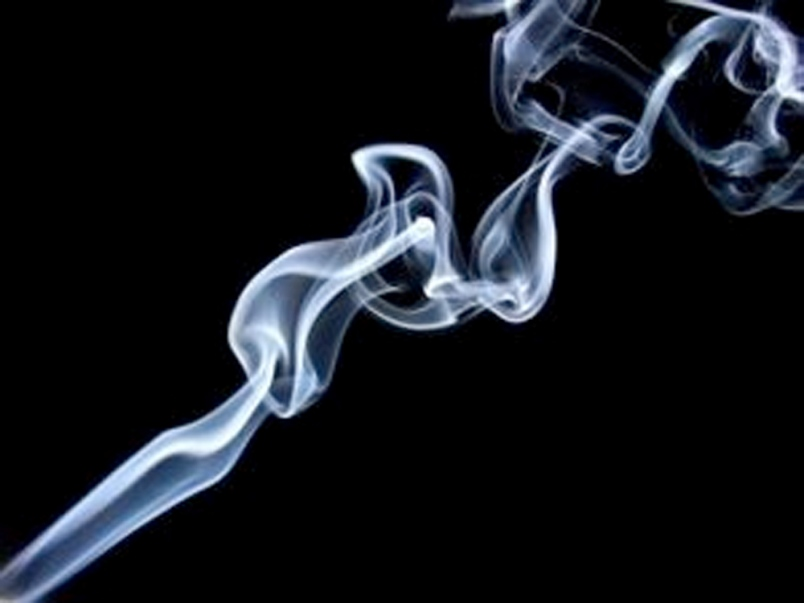
\includegraphics[width=0.5\textwidth]{images/smoke}
%https://www.google.se/search?client=ubuntu&q=cb+edits+smoke+png&tbm=isch&tbs=simg:CAQSlAEJkNL0D0I-7I0aiAELEKjU2AQaBAgVCAAMCxCwjKcIGl8KXQgDEiWoGUHnAegBsQw9sgxAlgawDIYnhSCHJ4okqzemIYgksCiVIKw3GjDJWGns8ZAx_17dvQFajhuRydFWdlJwDNo3VGI7iBUyNViewQZEJmiaYWGUhTUgxQOUgBAwLEI6u_1ggaCgoICAESBLt5JWoM&sa=X&ved=0ahUKEwiit7jKxKXZAhUBiCwKHTapCLQQ2A4IJygB&biw=1916&bih=948
\end{figure}


\subsection{The Boundary Layer}
In the context of fluid dynamics, the boundary layer studies the behavior of a fluid when it is flowing close to a solid surface. Imagine a laminar flow close to a solid surface; because of viscosity, the molecules flowing near the surface move slower, and, in the limit, the velocity of the molecules in direct contact with the surface is 0 (this is called the \emph{non-slip condition}). Thus, the velocity of the fluid increases smoothly, continuously and monotonously with the distance from the solid, until it reaches the \emph{free-flow} velocity, after which it stays constant. The region close to the surface, where the fluid moves slower, is called the \emph{boundary layer}, and is the region where the viscosity of the fluid influences its motion. Its height $\delta$ can be defined when the local velocity surpasses a certain threshold, such as 99\% of the free-flow velocity.

\begin{figure}
\caption{Turbulent boundary layer at the edge of a canal; the end of the BL is clearly visible, where the flow transitions from turbulent to laminar. Water flows from right to left.}
\label{fig:bl}
\centering
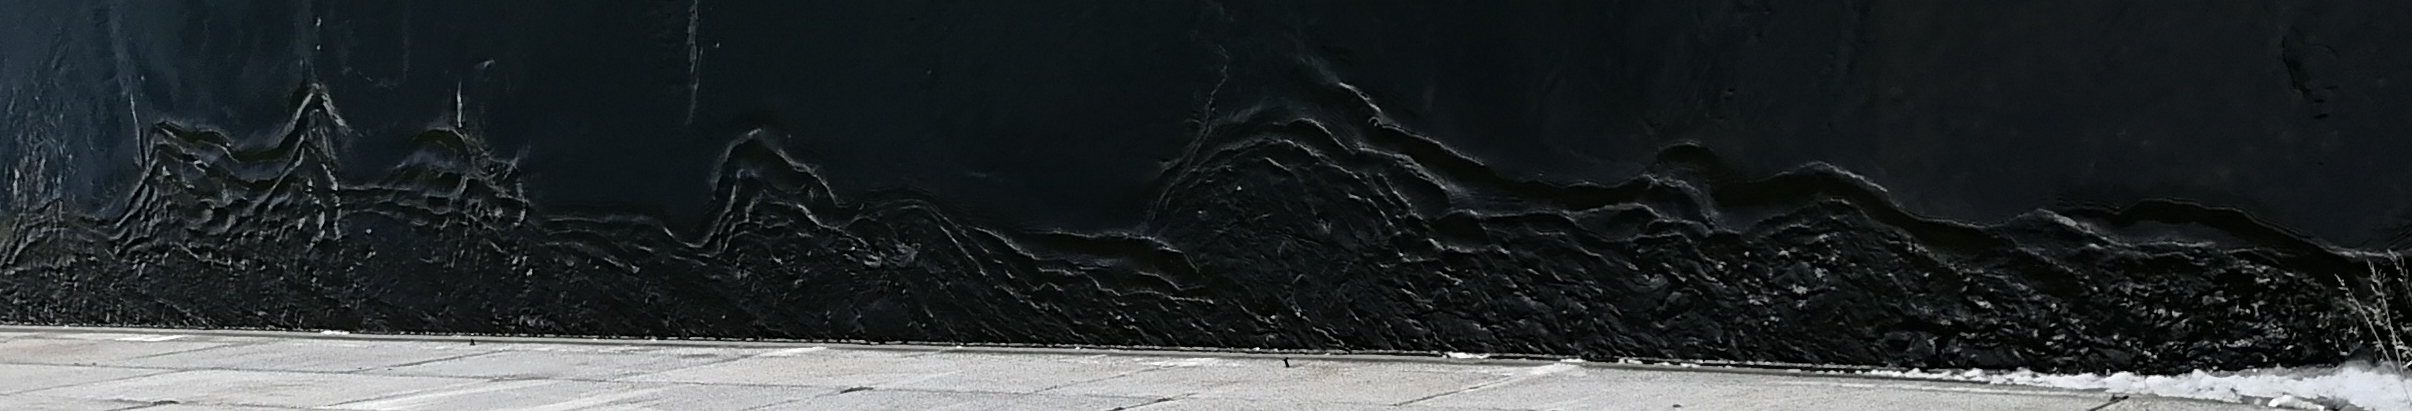
\includegraphics[width=\textwidth]{images/bl}
\end{figure}

The variation of velocity with distance from the surface, $\partial\overline{u}/\partial z$, is called \emph{shear}, and, together with viscosity, determines the materialization of turbulence in the flow. Every layer of fluid is squeezed between a faster moving layer above and a slower moving below; in high shear conditions, this causes high stress on the particles, and prevents them from moving orderly, thus leading to turbulent motion. Figure \ref{fig:bl} shows turbulence forming close to the wall in a canal, where the water flows from right to left. Viscosity and the no-slip condition prevent this phenomenon to arise in a region very close to the solid surface, called the \emph{laminar (or viscuous) sub-layer}, where we still find laminar motion.

The strength of the turbulence is proportional to $u_{rms}=(\overline{u'^2})^{1/2}$, which is, in turn, proportional to the shear. Again, because of the no-slip condition, $u_{rms}$ is zero at $z=0$, increases in the laminar sub-layer, and decreases to 0 at the end of the boundary layer, assuming laminar flow outside of it. Higher free-stream velocity generates higher shear, more turbulence, and a thinner laminar sub-layer. The strength of turbulence can be written in units of velocity, resulting in the \emph{friction velocity}, computed as $u_*=(\tau/\rho)^{1/2}=(\nu\cdot\partial\overline{u}/\partial z)^{1/2}$, where $\tau$ is the shear stress, $\rho$ is the density of the fluid, $\nu=\mu/\rho$ is the kinematic viscosity, and $\mu$ the dynamic viscosity. Therefore, the friction velocity increases with shear and viscosity, and decreases with density; it is proportional to the free-stream velocity and the turbulence strength, and inversely proportional to the height of the laminar sub-layer.

The mean velocity $\overline{u}$ increases linearly within the laminar sub-layer, then logarithmically until the end of the boundary layer, thus the shear decreases further away from the surface. In the logarithmic sub-layer, the velocity is computed as $\overline{u}(z)=u_*(\log z - \log z_0)/\kappa$, where $z_0$ is the characteristic roughness of the surface, and $\kappa$ is the von Karman's constant, whose value is around 0.4 [citation needed]. The characteristic roughness depends on the texture of the surface, and its relationship with the height $\delta_s$ of the laminar sub-layer; if the roughness scale is smaller than $\delta_s$, the logarithmic velocity profile is not affected by the texture, because the laminar sub-layer completely covers the variations on the surface, and we have the so-called smooth turbulent flow. If, on the contrary, the bumps in the surface are larger than $\delta_s$, the laminar sub-layer follow the profile of the surface, and the logarithmic velocity profile is altered depending on the texture, a regime called rough turbulent flow.

\section{The Atmospheric Boundary Layer}
The atmosphere is composed by air, which is behaves like fluid. Therefore, close to the Earth's surface, in the region called \emph{atmospheric boundary layer}, we find the same effects described in the previous section. Additionally, there are other phenomena that complicate things further, such as the temperature of the surface, which changes widely from day to night and from Summer to Winter, the rotation of the Earth, the varying roughness of the surface, due to cities and mountains, etc. The effect of the surface on the first few hundred meters of the atmosphere is the main focus of \emph{boundary layer meteorology}. 

The height of the atmospheric boundary layer (hereafter abbreviated as ABL) typically varies between 100 and 1000 meters, highly depending on the conditions, and it is always turbulent. There are three main instabilities driving turbulence in the ABL:

\begin{itemize}
\item Shear instability: caused by shear, the mechanism described in the previous section. This happens at high Reynolds number, and, by using typical values for the ABL, we find $Re$ well above $10^6$.
\item Kelvin-Helmholtz instability: occurs when there is a difference of density and velocity in different layers of flow. This is the mechanism that generates, for example, waves in ponds, lakes, and oceans.
\item Rayleigh-Bernard instability: is caused by the decrease of potential density\footnote{the potential density is the density that a parcel of air would attain if brought at a standard reference pressure adiabatically, i.e. disallowing exchanges of heat with its surroundings. Potential density is useful to compare densities irrespectively of pressure, i.e. altitude} with height, or, in other words, when warm fluid is below cold fluid; the warm fluid will rise, and the cold fluid will drop, a phenomenon called \emph{convection}. During hot Summer days, the surface is much warmer than the air, thus the air close to the surface will heat and tend to rise.
\end{itemize}

Turbulence has the very important role of transport and mix of air properties, such as heat, moisture, particles, aerosols, etc. This is especially true in \emph{unstable} conditions, when the air moving upwards (e.g. because it is warmer) is less dense than the air moving downwards; when the contrary happens, the ABL is called \emph{stable}.

The ABL can be divided in two main sub-layers: the inner surface layer and the outer Ekmann layer. This distinction is mainly done based on the scale of the dominating turbulent eddies: they are much smaller than the height of the ABL in the surface layer, and of comparable size in the outer layer.

It is very important to have a macroscopic understanding of the turbulent processes in the ABL, because they happen at length and time scales too small to be simulated in global climate models. The process of expressing the result of turbulence as a function of large scale parameters is called parametrization; having realistic models is essential in order to conduct precise simulations of the global climate in the scale of tens or hundreds of years, because errors tend to accumulate and amplificate as the simulation goes on. Other fields that benefit from the study of the ABL are urban meteorology (interested in the dispersion of pollutants), agricultural meteorology (interested in the formation of frost and dew, the temperature of the soil, etc.), aviation (predict fog and strong winds), and so on.

\subsection{Surface Fluxes}
A flux measures the amount of a physical quantity that flows through a surface. In the context of boundary layer meteorology, we are interested in the flows through the surface of earth, because, through them, the surface and the atmosphere exchange energy; these fluxes are thus measured in \si{\watt\per\square\meter}. The main source of energy for the surface is long-wave radiation coming from the sun, and short-wave radiation coming from the atmosphere and the clouds. A small amount of long-wave radiation is emitted from the surface, therefore let the net radiative flux be $R$, positive when the surface gains energy.

The main fluxes by which the surface loses energy to the atmosphere are called the turbulent flux of \emph{sensible heat} $H$, also called kinematic heat flux, and the turbulent flux of \emph{latent heat} $\lambda E$, also called kinematic flux of water vapor/moisture. The difference between the two is that the former causes an actual change of temperature, whereas the latter does not affect temperature\footnote{imagine a pot of boiling water; selecting a higher temperature on the stove will not increase the temperature of water above \SI{100}{\celsius}, but will make it boil faster. The additional heat introduced in the system is dissipated through increased evaporation}. The main causes of sensible heat fluxes are conduction and convection, whereas the main cause of latent heat fluxes is water movement: condensation, evaporation, melting, etc. 

The final flux of interest is the soil heat flux $G$, which is simply the heat "absorbed" by the surface and not given to the atmosphere. These four fluxes are linked by the surface energy balance equation:

$$
R=H+\lambda E+G
$$

which states that the total incoming energy $R$ must be equal to the energy given back to the atmosphere $H+\lambda E$ (not counting long-wave radiation, which is accounted to in $R$) plus the energy absorbed by the surface $G$.

The turbulent fluxes $H$ and $\lambda E$ are constant in the surface layer [todo add citation]. Experimentally, the energy balance is not always achieved [todo cite from cabauw] due to difficulty in measuring fluxes due to eddy correlation being inaccurate (verify this)

\subsection{The Turbulence Kinetic Energy Budged}
Kinetic energy is energy stored in form of movement: faster or heavier objects have more kinetic energy than slower or lighter ones. The Reynolds decomposition allows us to decompose the kinetic energy of turbulent flows in two terms: one caused by the mean flow, and one caused by turbulence. This decomposition can be justified by examining the temporal spectrum of kinetic energy, shown in figure \ref{fig:tkespectrum}. Four peaks are visible, corresponding to different sources of kinetic energy: turbulence, day-night cycle, westerlies\footnote{winds blowing from the east towards the west in the mid-latitudes}, and seasons. Importantly, there are few sources of kinetic energy in the 30 minutes to one hour time scale; this so-called spectral gap allows us to separate between turbulence and other sources of fluctuations in the atmosphere.

\begin{figure}
\caption{Change of atmospheric kinetic energy at different time-scales. The peaks in the scale of days and months and years are due to the day-night and Summer-Winter cycles, the peaks in the monthly scale are due to baroclinic instability in the mid-latitude westerlies, and the peaks at one minute are due to convection and atmospheric turbulence \citep{tkespectrumsrc,tkespectrumorig}}
\label{fig:tkespectrum}
\centering
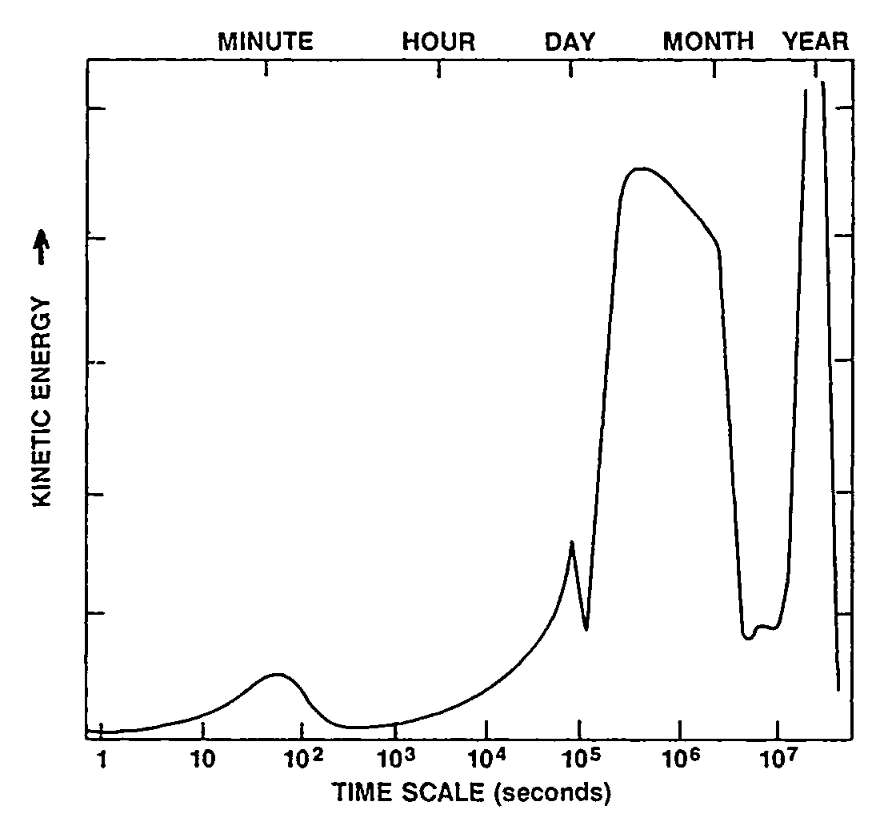
\includegraphics[width=0.5\textwidth]{images/kinetic_energy_spectrum}
\end{figure}

From now on, we will use a coordinate system with the $x$ axis aligned to the average horizontal wind direction, the $y$ axis perpendicular to it, and the $z$ axis pointing away from the surface. Then, we will use the letters $u$, $v$ and $w$ to denote the components of the wind along the axes $x$, $y$ and $z$ respectively; clearly, $\overline{v}=0$. Eddy fluxes can then be described in terms of covariances: let $\theta$ denote the potential temperature\footnote{the potential temperature is final temperature after bringing a parcel of air to a standard pressure adiabatically, i.e. not allowing exchange of temperature with the surroundings. It is a useful mean to compare temperatures irrespectively of pressure, i.e. altitude}, then $\overline{w'\theta'}$ is the turbulent heat flux, i.e. the sensible heat flux in the vertical due to wind. Usually the ABL  studied assuming homogeneous horizontal conditions, because they vary on a length scale larger than the height of the ABL. Because of this, the horizontal eddy correlations $\partial\overline{u'a'}/\partial x$ and $\partial\overline{v'a'}/\partial y$ are usually of negligible intensity, and are thus ignored. Note that this is not necessarily true when clouds are involved.

It is important to notice that turbulence is dissipative in nature. Consider a hot Summer day, where air is warmer close to the surface, and a circular eddy moving some air up and some down, so that the average motion is zero. The parcel of air moving up ($w'>0$) ends up being warmer than its surroundings ($\theta'>0$), while the one moving down ($w'<0$) will be colder ($\theta'<0$); the result is a new transport of heat through the eddy: $\overline{w'\theta'}>0$. On the contrary, imagine a cold night, where the air close to the surface is colder; the same eddy would transport a colder parcel of air upwards, and a warmer one downwards. In both cases, the end result would be a net transport of heat without transport of mass. Because of the ??? law, the eddy must lose energy, and thus dissipate over time.

Since turbulence changes over time, we are more interested in the change of kinetic energy, the \emph{turbulent kinetic energy budget}. A full derivation is out of the scope of this work, but its final form \citep{basicatm} can be derived from prime physical principles, resulting in

\begin{equation}
\frac{\partial\overline{{e'}^2}}{\partial t}
=\underbrace{\overline{u'w'}\frac{\partial\overline{u}}{\partial z}}_P
-\underbrace{\frac{g}{T}\overline{w'\theta'}}_B
+\underbrace{\frac{\partial}{\partial z}\frac{\overline{w'{e'}^2}}{2}}_{T_t}
+\underbrace{\frac{1}{\rho}\frac{\partial\overline{p'w'}}{\partial z}}_{T_p}
+\epsilon
\end{equation}

Where ${e'}^2={u'}^2+{v'}^2+{w'}^2$. The $P$ term is the production due to shear, $B$ is the production due to buoyancy, $T_t$ is the turbulent transport of TKE by large-scale eddies, $T_p$ is the transport due to pressure, and $\epsilon$ is molecular dissipation due to viscosity. $P$ and $B$ are the most prominent terms, and the transport terms are close to zero in neutral conditions.

TODO elaborate on 3.4, 3.5 (reason why P and B have opposite sign), 3.6, 

\subsection{Monin-Obukhov Similarity Theory}
\label{sec:most}
One of the factors to distinguish laminar from turbulent flow is the length scale $L$ of the system. This length scale for the ABL was derived by A. M. Obukhov in 1946, and forms the basis of the similarity theory. According to this theory, the normalized wind and temperature profiles can be expressed as an unique function of $\xi=z/L$:

\begin{equation}
\label{eq:most_l}
L=-\frac{u_*^3}{\kappa\frac{g}{\theta_v}\frac{Q}{\rho c_\rho}}
=-\frac{u_*^3 T_v}{\kappa g \overline{w'\theta_v}}
\end{equation}

\begin{equation}
\label{eq:phi_m}
\frac{\partial\overline{u}}{\partial z}\frac{kz}{u_*}=\phi_m(\xi)
\end{equation}

\begin{equation}
\label{eq:phi_h}
\frac{\partial\overline{\theta_v}}{\partial z}\frac{kz}{T_*}=\phi_h(\xi)
\end{equation}

With

\begin{itemize}
\item $g=\SI{9.81}{\meter\per\square\second}$ the acceleration due to Earth's gravity
\item $\kappa=0.4$ the von Karman constant

\item $\theta_v$ virtual temperature\footnote{potential temperature of dry air if it had the same density as moist air. It allows to use formulas for dry air when the air is not dry.}, obtained as

\begin{equation}
\label{eq:vtemp}
\theta_v=\theta\frac{1+r_v/\epsilon}{1+r_v}=\theta(1+0.61\cdot q)
\end{equation}

Where $\theta$ is the air temperature, $r_v$ is the mixing ratio, $q=r_v/(1+r_v)$ the specific humidity, and $\epsilon$ is the ratio of the gas constants of dry air and water vapor, roughly 0.622.

\item $\rho$ the air density, computed from the pressure $P$ and the specific gas constant for dry air $R=\SI{287.058}{\joule\per\kilo\gram\kelvin}$ as

$$
\rho=\frac{P_0}{RT_v}
$$


\item $c_\rho$ specific heat of dry air, \SI{1005}{\joule\per\kilo\gram\per\kelvin} at \SI{300}{\kelvin}
\item $Q$ the buoyancy flux, approximated by $H+0.07\lambda E$ and measured in \si{\watt\per\square\meter}
\item $\overline{w'\theta_v}=Q/\rho c_\rho$ the flux of virtual potential temperature, measured in \si{\kelvin\meter\per\second}
\item $T_*=-\overline{w'\theta}/u_*$
\end{itemize}

The stability parameter $\xi$ is positive for stable conditions, where wind shear dominates the production of TKE, and negative for unstable conditions, where buoyancy is the main contributor to turbulence. It approaches 0 in the limit of neutral stratification (i.e. $\partial\overline{\theta}/\partial z=0$), because the temperature flux goes to 0 causing $L$ go to infinity.

The universal functions $\phi_m$ and $\phi_h$ must be determined experimentally. This is no easy task, and considerable effort has been devoted to it; one of the greatest difficulties lies in obtaining accurate and unbiased measurements, especially the fluxes. \cite{hogstrom88} is a meta-study that aggregates and improves many previous results, and suggests the following expressions:

\begin{align}
\phi_m(\xi)&=\begin{cases}
\mathrlap{(1-19.3\xi)^{-1/4}} \hphantom{0.95(1-11.6\xi)^{-1/2}} & -2<\xi<0 \\
1+6\xi & 0<\xi<1\\
\end{cases} \\
\phi_h(\xi)&=\begin{cases}
0.95(1-11.6\xi)^{-1/2} & -2<\xi<0 \\
0.95+8\xi & 0<\xi<1
\end{cases}
\end{align}

The Monin-Obukhov similarity theory is only applicable in the surface layer, at heights much larger than the aerodynamic roughness length, and with $\vert\xi\vert<2$; even under ideal conditions, the predictions of this theory are accurate up to 10-20\% [foken 2006].

\section{Machine Learning}
The goal of Machine learning is to develop algorithms that allow computers to learn from examples. Learning is intended as the ability of inferring general rules from the available examples, so that new, previously unseen examples can be correctly characterized. The set of samples from which the computer is supposed to learn is called the \emph{training set}, and each sample is a sequence of numbers describing its attributes, or \emph{features}. There are three approaches in machine learning:

\begin{itemize}
\item \emph{Supervised} learning: in this setting, the examples are composed of an input and a desired output, and the goal is to build a model that can correctly predict the output given the input. There are different algorithms depending on the type of output: \emph{regression} algorithms predict continuous output, while \emph{classification} algorithms predict discrete output.

\item \emph{Unsupervised} learning: in this setting, no output is available. The task of the algorithm is to figure out hidden relationships between the samples in the training set, for example whether they form clusters, or there are anomalous samples, or the correlation between features of the examples.

\item \emph{Reinforcement} learning: in this setting, the computer is free to act in an environment and to observe how the environment responds to its actions. Additionally, it receives a \emph{reward} for every action it takes, and the goal of the computer is to learn a sequence of actions that maximizes the received reward. Reinforcement learning is often applied in robotics [citation] and game playing [alphazero citation].
\end{itemize}

A supervised machine learning model uses a set of parameters to compute the output value starting from the input features. The actual parameters values are learned from the training set in a process called \emph{training}. This process is controlled by another set of parameters called hyper-parameters, whose value can be found from the training data as well. Whereas the parameters control the relationship between input and output, hyper-parameters control the "character" of the learning algorithm, such as how eager or conservative it is in learning minute details in the features. Learning too many details can be detrimental, because some differences can be due to noise, rather than actual differences.

The next sections describe the theory of learning, a general technique to estimate the parameters of a regression model, and introduce several machine learning algorithms for regression.

\paragraph{Notation:} Scalars are denoted in \textit{italic}, vectors (always column) and matrices in \textbf{bold}. The training set contains $N$ training samples, indexed by $n$, and each sample is a pair of feature vector $\bm x_n\in\mathbb{R}^D$ and a target value $t_n\in\mathbb{R}$. The feature vectors are grouped in the $N\times D$ matrix $\bm X=\left[\bm x_1\dotsb\bm x_N\right]^\intercal$ and the target values in the $N\times 1$ vector $\bm t=\left[t_1,\ldots,t_n\right]^\intercal$. Models are parametrized by a parameter vector $\bm\theta$ and their output for the feature vector $\bm x_n$ is $f_n=f(\bm x_n;\bm\theta)$. The vector containing both parameters and hyper-parameters is denoted with $\bm\Theta$.

\subsection{Learning Theory}
The goal of supervised learning is to use the training examples $D=(\bm X, \bm t)$, independent and identically distributed according to an unknown distribution $p_{XT}$, to find a good prediction rule $\hat{f}:\mathcal{X}\rightarrow\mathcal{Y}$ among a family of available functions $\mathcal{F}$. In most practical cases, $\mathcal{X}=\mathbb{R}^D$ and $\mathcal{Y}$ is either $\mathbb{R}$ for regression or a subset of $\mathbb{N}$ for classification. The goodness of a prediction rule $f$ is measured through a \emph{loss function} $\ell:\mathcal{Y}\times\mathcal{Y}\rightarrow\mathbb{R}$ that tells, given a target value $t$ and a guess $y=f(x)$, how much the guess is off. The \emph{risk} of an estimator $f$ is simply its expected loss:

\begin{equation}
R(f)=\mathbb{E}_{(x,t)\sim p_{XT}}\left[\ell(f(x),t) \vert f \right]
\end{equation}

The ideal situation is to find the estimator $f^*$ that has the lowest risk; unfortunately this is not possible, because the distribution $p_{XT}$ is unknown. Since the training data is a sample from this distribution, we can compute the \emph{empirical risk} of $f$ on this set of examples instead:

\begin{equation}
\hat{R}(f)=\mathbb{E}_{(x,t)\sim D}\left[\ell(f(x),t)\vert f\right]=\frac{1}{N}\sum_{n=1}^N \ell(f(x_n),t_n)
\end{equation}

We can now use the empirical risk as a surrogate for the true risk, selecting the estimator

\begin{equation}
\hat{f}=\argmin_{f\in\mathcal{F}}\hat{R}(f)
\end{equation}

as our best guess. This procedure is called \emph{empirical risk minimization}. Note that $\hat{f}$ is a random function, because it depends on $D$, which is a random variable. An interesting question to ask is how good $\hat{f}$ actually is, or, in other words, what is its expected true risk $\mathbb{E}[R(\hat{f})]$ and how it compares to the lowest attainable risk $R(f^*)$. This latter quantity can be decomposed as

\begin{equation}
\mathbb{E}[R(\hat{f})]-R(f^*)=
\left(\mathbb{E}[R(\hat{f})]-\inf_{f\in\mathcal{F}} R(f)\right)
+\left(\inf_{f\in\mathcal{F}} R(f)-R(f^*)\right)
\end{equation}

Where the first term is the \emph{estimation} error incurred by not selecting the best possible estimator in $\mathcal{F}$, and the second term is the \emph{approximation} error caused by searching a good estimator in $\mathcal{F}$. They usually have opposite behavior:

\begin{itemize}
\item the estimation error is high when $\mathcal{F}$ is too complex for the data at hand, where complexity refers to the range of phenomena that can be accurately modeled by these functions. In other words, $\mathcal{F}$ contains many valid explanations that are equally good on the training set (they have low empirical risk $\hat{R}$), but are not accurate models of the underlying phenomenon $p_{XT}$, i.e. they do not generalize well (they have high risk $R$);
\item the approximation error is high when $\mathcal{F}$ cannot adequately model the phenomenon that we are trying to describe, i.e. when it does not contain any good explanation for it.
\end{itemize}

This decomposition is often referred to as the \emph{bias-variance decomposition}, where bias and variance refer to, respectively, approximation and estimation error.

The fundamental problem is to find a class of functions that is powerful enough to model $p_{XT}$, but not too powerful so as to contain too many good explanations, because we would not be able to choose. Equivalently, we want to find a good model, one that can explain the data we have, and generalize to new examples. This problem is known as \emph{model selection}, and is important to distinguish between model selection for \emph{identification}, and model selection for \emph{estimation}. In the former case, the goal is to obtain a model and its parameters, to be used on new prediction problems, whereas the goal of the latter is to obtain a realistic estimate of the performance that can be obtained on new data. This problem can be approached in two ways: by directly estimating approximation and estimation errors using hold-out sets, or by penalizing complex models in order to favor simpler explanations, even though they might have slightly higher empirical risk. The next sections describe these two approaches.


\subsection{Cross Validation}
\label{sec:cv}
The idea behind hold-out methods is to partition the available data in two smaller sets $D_T$ and $D_V$, usually of size 2/3 and 1/3 of the total, and use the \emph{training} set $D_T$ to choose $\hat{f}$ and $D_V$ to estimate its risk. Since $D$ is assumed to be a representative sample from $p_{XT}$, if the two partitions contain independent and identically distributed samples, the empirical risk on the \emph{validation set} $D_V$ can give us a glimpse on the generalization power of $\hat{f}$. This is because the validation set contains new samples that were not used to choose $\hat{f}$, thus the empirical risk on this set is an unbiased estimate of the true risk of the discovered model. This allows us not only to be confident about the performance of the estimator on unseen data, but also to compare different estimators. The problem of a single hold-out set is the variance of its estimate of the risk, which depends on the size of the validation set. This means that we are faced with a trade-off: use a lot of data to select a good estimator, but have high uncertainty in its estimated performance, or use less data and select a less powerful estimator, but have a more accurate picture of its performance.

The solution to this problem is to repeatedly perform this partitioning procedure so as to obtain many estimates of the risk, each on a different subset of validation samples, and average these results together. This can be done in a number of different ways:

\begin{itemize}
\item in random subsampling, the procedure above is simply repeated many times, by using two thirds random examples for training, and the remaining one third for validation;
\item In bootstrapping \citep{bootstrap}, the training set is created by taking $N=\vert D\vert$ examples \emph{with replacement} from $D$, and using the remaining examples for validation. This means that the validation set contains on average approximately 36.8\% of the samples in $D$, and the training set the remaining 63.2\%, with many duplicates;
\item In k-fold cross validation \citep{kfold}, $D$ is partitioned in $k$ subsets, and each of them is used in turn as validation set, while the others are used for training. This produces $k$ estimates of the true risk, coming from the $k$ subsets.
\end{itemize}

Regardless of the method used, the final estimate of the performance is the average of the estimates obtained from the individual trials. Every method has different properties regarding both the bias and the variance of the estimates, and there is considerable controversy on which method should be used in which situation. For example, \cite{cv_bootstrap} recommends using 10-fold cross validation for comparing models, because, although its estimate of the performance is biased, it has lower variance compared to bootstrapping; however, \cite{no_unbiased_cv} show that it is not possible to obtain an universal unbiased estimate of the variance of k-fold cross validation. \cite{cvmyths} further discusses this issue, and debunks some myths and commonly held misconceptions about cross validation, including the belief, consequent \cite{cv_bootstrap}, that 10-fold cross validation is always the best choice. Generally, there is a tradeoff in choosing the value of k, as high values yield estimates with lower bias, but higher variance \citep{cv_survey}, and are more computationally intensive.

nested cv \cite{nested_cv}

\subsection{Parameter Estimation for Regression}
\label{sec:regression_fit}

In this section, we describe a general framework, rooted in Bayesian statistics, for estimating the parameters of a regression model, while controlling overfitting. An advantage of Bayesian methods is that they offer a sound theoretical foundation for model selection, without requiring repeated experiments to choose among candidate models, although this mathematical rigor is not free from practical difficulties \citep{bayesian_model_selection, practical_bayesian_model_selection}.

A common assumption in the regression setting is that the observations are corrupted by additive Gaussian white noise, i.e. $t_n=y_n+\epsilon_n$, where $y_n$ is the "true" value, and $\epsilon_n\sim\mathcal{N}(0,\beta^{-1})$ is the noise. Let $f_n=f(\bm x_n;\bm{\theta})$ be the model's prediction for the sample $\bm x_n$, then we can write the probability of observing $t_n$, assuming that $f_n=y_n$, as:

\begin{equation}
p(t_n\vert \bm{x_n},\bm\Theta)=\mathcal{N}(t_n\vert f(\bm{x_n};\bm\theta),\beta^{-1})
\end{equation}

This probability is called \emph{likelihood} of the observation $t_n$, under the model $f(\cdot;\cdot)$ with parameters $\bm{\theta}$. Since the training data is assumed to be independent and identically distributed, the likelihood of the whole training set is

\begin{equation}
\label{eq:likelihood}
p(\bm{t}\vert\bm{X}, \bm\Theta)=\prod_{n=1}^N  \mathcal{N}(t_n\vert f(\bm{x_n};\bm\theta),\beta^{-1})
\end{equation}

And the predicted value $t$ for a new sample $\bm x$ is distributed as

\begin{equation}
p(t\vert \bm x, \bm X, \bm t)=\int
p(t\vert\bm x,\bm\Theta)\cdot p(\bm\Theta\vert \bm t, \bm X)\ \text{d}\bm\Theta 
\end{equation}

In practice, it is not feasible to compute this integral, and its value is dominated by the values of $\bm\theta$ close to the one that maximizes equation \ref{eq:likelihood} anyways; this is the gist of \emph{maximum likelihood estimation} (MLE). Note that, since the goal is to predict $y_n$, there is a high probability that the "true" parameters would \emph{not} be the ones with maximum likelihood. When a model learns the noise in the training data, it cannot generalize well to new, unseen data, because the noise is random. This situation is known as \emph{overfitting}, and tends to happen when the model is too complex relative to the amount of data available for training, and is related to high estimation error mentioned previously.

The risk of overfitting can be reduced with a number of \emph{regularization} strategies. A widely used strategy consists in including a prior distribution on the parameters of the model, and maximizing their posterior distribution, computed using Bayes theorem:


\begin{align}
\begin{split}
\label{eq:map}
p(\bm\Theta\vert\bm t, \bm X)&=\frac{p(\bm X, \bm t\vert\bm\Theta)\cdot p(\bm\Theta)}{p(\bm X, \bm t)}\\
&\propto p(\bm t\vert \bm X,\bm\Theta)\cdot p(\bm X\vert\bm\Theta)\cdot p(\bm\Theta)\\
&\propto p(\bm t\vert \bm X,\bm\Theta)\cdot p(\bm\Theta)
\end{split}
\end{align}


where we removed $p(\bm X,\bm t)$ and $p(\bm X\vert\bm\Theta)=p(\bm X)$ because they are constant for a given dataset, and we are not interested in the exact probability, but where it reaches its maximum value. This parameter estimation procedure is called \emph{maximum a posteriori} (MAP). Two commonly used prior distributions are the multivariate Laplace and the multivariate Normal, leading respectively to L1 and L2 regularization, when centered and symmetrical/spherical.

The maximization of the posterior can be done conveniently by maximizing its logarithm; this gives expressions that are easier to handle analytically, and give less numerical problems when computed. The MAP problem can be formulated as follows:

\begin{equation}
\bm\Theta^*=\argmax_{\bm\Theta}\ \log p(\bm t\vert\bm X,\bm\Theta)+\log p(\bm\Theta)
\end{equation}


If we assume a Gaussian likelihood like the one in equation \ref{eq:likelihood}, and a spherical Normal prior distribution $p(\bm\theta)=\mathcal{N}(\bm 0, \lambda\bm I)$, the MAP estimation of equation \ref{eq:map} becomes, after removing unnecessary constant terms,

\begin{equation}
\label{eq:least_squares}
\bm\theta^*=\argmin_{\bm\theta}\ L(\bm\theta)=\argmin_{\bm\theta}\sum_{n=1}^N\left( f(\bm x_n,\theta)-t_n\right)^2+\lambda\bm\theta^\intercal\bm\theta
\end{equation}

Where $L$ is the \emph{loss function}, in this case the sum-of-squares error. It is customary to use the mean squared error instead of the sum of squares because it results in smaller numbers and is readily interpreted; being only a constant factor away from \ref{eq:least_squares}, it does not transcend the essence of MAP estimation. The parameter $\beta$ can be estimated as well in a similar way, if necessary, and a fully Bayesian treatment allows to estimate $\lambda$, too. Depending on the model $f(\bm x_n,\bm\theta)$, \ref{eq:least_squares} can be solved analytically to yield a closed-form solution for $\bm\theta$.
 
When this is not possible, iterative optimization methods are employed. A widely used approach is called \emph{gradient descent}: the gradient of a function computed at a given location "points" to the steepest direction where the function's value increases. By repeatedly following the gradient, it is possible to reach a local maximum, and, in the opposite direction, a local minimum:

\begin{equation}
\bm\theta_{n+1}:=\bm\theta_n-\eta\cdot\nabla f(\bm x_n)
\end{equation}

the series $\bm\theta_1,\ldots,\bm\theta_n$ is guaranteed to converge to the local optimum at a rate of $O(n^{-1})$ if certain conditions are met \citep{gd_convergence}. \cite{numopt} describes more advanced optimization techniques that use the gradient and, possibly, the Hessian, such as Newton's. The gradient of $L(\bm\theta)$ is

\begin{equation}
\label{eq:least_squares_gradient}
\nabla_{\bm\theta}\log p(\bm\theta\vert\bm t,\bm X)
=2\sum_{n=1}^N \big(f(\bm x_n;\theta)-\bm t_n\big)\cdot\nabla_{\bm\theta}f(\bm x_n;\theta) + 2\lambda\bm\theta
\end{equation}

And its Hessian is

\begin{equation}
\label{eq:least_squares_hessian}
\nabla^2_{\bm\theta}\log p(\bm\theta\vert\bm t,\bm X)=2\sum_{n=1}^{N}\bigg[
\big(\nabla_{\bm\theta} f(\bm x_n;\bm\theta)\big)
\big(\nabla_{\bm\theta} f(\bm x_n;\bm\theta)\big)^\intercal
+\big(f(\bm x_n;\bm\theta)-t_n\big)\nabla^2_{\bm\theta}f(\bm x_n;\theta)\bigg]+2\lambda\bm I
\end{equation}

In some cases, the gradient and the Hessian can be approximated using a random subset of the training set, and, in extreme cases, a single sample. These variants are called \emph{minibatch} gradient descent and \emph{stochastic} gradient descent respectively. They both compute a noisy approximation to the true gradient, which can actually improve convergence and generalization of high-dimensional, non-convex loss functions such as those found in deep learning \citep{sgd_noise, bayesian_sgd}. Vanilla gradient descent can be greatly improved with a number of techniques, such as momentum \citep{gd_momentum}, adaptive learning rate \citep{adagrad, adadelta, adam}, and so on, see \cite{gd_overview} for an overview. 

\subsection{Hyperparameter Optimization}
grid search vs random search

\subsection{Ridge Regression}
A linear regression model has the form $f(\bm x_n;\bm\theta)=\bm\theta^\intercal\bm x_n$; ridge regression is simply L2-regularized linear regression. This model is simple enough that the solution for equation \ref{eq:least_squares} can be found analytically in closed form:

\begin{equation}
\label{eq:ridge_solution}
\bm\theta^*=(\bm X^\intercal\bm X+\lambda\bm I)^{-1}\bm X^\intercal\bm t
\end{equation}

Notice that the term \emph{linear} in linear regression refers to linearity with respect to the parameters, not the features. In fact, new features can be added through the use of a possibly non-linear feature mapping $\phi:\mathbb{R}^D\rightarrow\mathbb{R}^M$, such that $\bm x^\prime_n=\phi(\bm x_n)=\left[\phi_1(\bm x_n),\ldots,\phi_M(\bm x_n)\right]^\intercal$. Then, the model parameters can be fitted to the augmented training set $\bm X^\prime$. A typical feature added is a bias $\phi_1(\bm x)=1$.

\subsection{k-Nearest Neighbors}
The k-nearest neighbor model \cite{knn} predicts a value for a sample $\bm x$ by averaging the target values of the $K$ training samples that are closest to $\bm x$, possibly weighted by distance or some other metric. Let $\bm t_{(1)},\ldots,\bm t_{(k)}$ be the target values of the $K$ training samples closest to $\bm x$ according to a distance metric $d:\mathbb{R}^D\rightarrow\mathbb{R}$, then we have

\begin{equation}
f(\bm x)=\sum_{k=1}^K w_{(k)}\cdot\bm t_{(k)}
\end{equation}


Note that the k-nearest neighbors algorithm does not have parameters, only hyper\hyp{}parameters: $K$ itself, the distance function, and the weighting scheme. Typical distance functions are the Manhattan distance $d(\bm u,\bm v)=\sum_{d=1}^D\vert u_d-v_d\vert$ and the squared Euclidean distance $d(\bm u,\bm v)=\sum_{d=1}^D(u_d-v_d)^2$, and typical weights are uniform $w_{(k)}=1/K$ and based on distance $w_{(k)}=d(\bm x,\bm x_{(k)})/\sum_{k^\prime=1}^K d(\bm x,\bm x_{(k^\prime)})$.

\subsection{Random Forests}
Random forests are an ensemble approach to prediction whose output values are the combination of the output of multiple decision trees \cite{random_forests}. In general, ensemble methods improve the performance of a single model by combining the output of many models trained on random subsets of features and/or samples.

A decision tree is a sequence of nested \emph{if-then-else} rules, each of them testing one of the features of the input sample: inference starts from the root, and successively traverses each node by moving to the correct child, until a leaf, containing the final prediction, is reached. For classification, the prediction is the most frequent class among the training samples that end up in that leaf, while for regression the output value can be their average, or the output of a more complicated regression model trained on those samples.

Given a training set, many decision trees can be built using different random subsets of features. This creates a number of \emph{expert} trees, each of them specialized in a restricted domain of the data. No tree is good enough on its own as it overfits its domain, but by averaging the output of many decision trees, their errors tend to cancel out.

A simple and widely used algorithm for building decision trees is CART \citep{cart}. It builds decision trees by greedily and recursively partitioning the training samples until a stopping criterion is met. Partitions are created by selecting the split that has the smallest impurity; a common measure for regression is the mean squared error, while Gini impurity or cross-entropy are popular options in classification. Let $X$ be a set of training samples and $\Sigma=(f,\tau)$ be a candidate split on feature $f$ with threshold $\tau$, then we can partition the training samples in two sets:

\begin{align}
S^-(\Sigma)&=\{\bm x\in X\vert \bm x_f\leq\tau\} \\
S^+(\Sigma)&=\{\bm x\in X\vert \bm x_f>\tau\}
\end{align}

And define the impurity $I$ of $\Sigma$ as the weighted average of the impurities of the two sets:

\begin{equation}
I(\Sigma)=\frac{\vert S^-(\Sigma)\vert}{\vert X\vert}I(S^-(\Sigma))+\frac{\vert S^+(\Sigma)\vert}{\vert X\vert}I(S^+(\Sigma))
\end{equation}

The best split is then

\begin{equation}
\Sigma^*=\argmin_{\Sigma}\ I(\Sigma)
\end{equation}

This best split defines a new node in the tree, and the construction can proceed recursively on its two children $S^-(\Sigma^*)$ and$ S^+(\Sigma^*)$. Stopping criteria for the construction can be a minimum impurity $I(X)$, a minimum impurity decrease with respect to the parent $I(X) - I(\Sigma^*)$, or a minimum cardinality for $X$ or the two splits $S^+$ and $S^-$.

\subsection{Gaussian Processes}
todo

\subsection{Neural Networks}
todo

\chapter{Method}

\section{Data Collection}
\label{sec:data_collection}
The Cabauw Experimental Site for Atmospheric Research\footnote{\url{http://www.cesar-database.nl/}} (Cesar) is a consortium formed by eight Dutch institutes and universities, which collaborate to operate and maintain an observatory for micro-meteorological conditions near the village of Cabauw, the Netherlands. The data collected characterizes the state of the atmosphere and the soil, and their interaction via radiation and surface fluxes.

The observatory is surrounded by fields and no urban agglomerations is present within 15 kilometers; the land is flat with changes of altitude within a few meters over 20 kilometers. The main mast is 213 meters high and offers measurement levels every 20 meters; at each level there are three booms of length 10 meters that allow observations unobstructed by the main mast. There are three additional smaller masts of height 10 and 20 meters located close to the main mast, in order to obtain undisturbed measurements at the lower levels, and facilities to perform soil and surface observations.

The main focus of this project is on wind and temperature profiles, and the turbulent fluxes of sensible and latent heat. Additional variables, such as temperature and humidity, are needed to compute quantities of interest, most importantly the Obukhov length, and as possible predictors for the universal functions. There is one measurement for each variable every ten minutes, and missing measurements are gap-filled with a number of techniques. The data collected is always visually validated by an operator, which marks suspect or invalid sections of data

The Cesar observatory provides full information regarding data collection\footnote{\url{http://projects.knmi.nl/cabauw/insitu/observations/documentation}}, what follows is a brief summary of the most relevant sections.

\begin{figure}
\caption{Sonic anemometer to measure wind and optical open-path sensor to measure humidity at the 180m level of the Cabauw mast.}
\label{fig:bl}
\centering
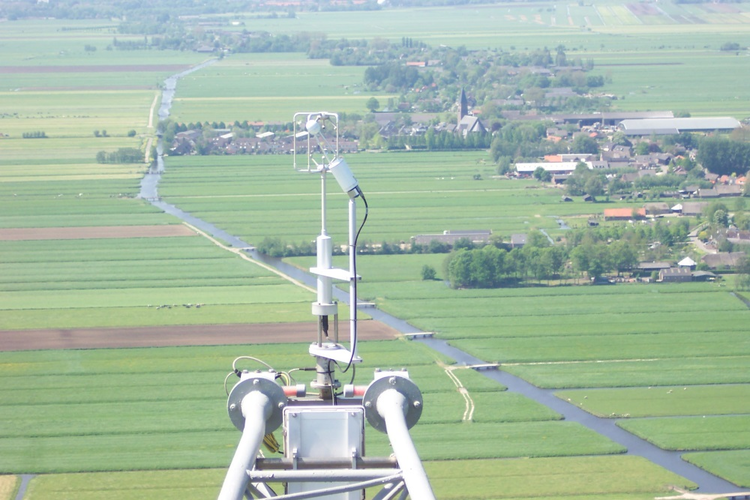
\includegraphics[width=0.75\textwidth]{images/cabauw_turbulence_instruments}
% https://www.knmi.nl/research/observations-data-technology/projects/cabauw-in-situ-measurements
\end{figure}

\subsection{Wind Measurement}
Wind speed and direction are measured at heights of 200, 140, 80, 40, 20 and 10 meters, in either two or all three booms available. The wind vane that measures direction has a resolution of $1.5^\circ$, and the cup anemometer that measures wind speed has an accuracy of the largest between 1\% and \SI{0.1}{\meter\per\second}. \cite{windinstr} studied the threshold sensitivity of both instruments, and fount it lower than \SI{0.5}{\meter\per\second}, even though the measurements are inaccurate up to \SI{3}{\meter\per\second}.

For every ten minutes interval, the measurement comes from the instrument that is best exposed to the wind, and less affected by the obstruction caused by the mast. Corrections are then applied to the raw measurements to further attenuate the disturbance by the tower, following \cite{winddistortion}.

\subsection{Air Temperature Measurement}
Air temperature is measured at heights of 200, 140, 80, 40, 20, 10 and 1.5 meters. todo write more

\subsection{Eddy Correlation}
\label{sec:eddy_correlation}
The eddy correlation technique is used to compute the turbulent surface fluxes of sensible and latent heat, as well as momentum and $CO_2$, starting from fluctuations in wind, temperature, and humidity.

These measurements are obtained with, respectively, a sonic anemometer, a sonic thermometer, and an optical open-path sensor. Sonic anemometers measure the wind speed by leveraging the fact that the speed of sound in free air is affected by the speed of the air itself; since the speed of sound is known, the wind speed can be easily recovered from the time a sound impulse takes to travel a short distance. By measuring the wind velocity along three orthogonal paths, the full wind vector can be recovered. Sonic thermometers work similarly, by leveraging the fact that the speed of sound is affected by the temperature of the medium it travels in. These instruments can take up to 100 measurements per second. Optical open-path sensors quantify the amount of water vapor and carbon dioxide in the air by emitting a ray of infrared light and measuring its intensity 10 to 20 centimeters further away. $H_2O$ and $CO_2$ molecules in the air absorb electromagnetic radiation at known frequencies, thus the concentration of water vapor and carbon dioxide can be inferred by measuring the attenuation at these wavelengths.

The eddy correlation technique measures fluxes by computing their sample covariance with the vertical wind speed. Let $w_t$ be the vertical wind speed at time $t$, then the turbulent vertical flux for the quantity $a$ is computed as follows:

$$
F_a=\frac{1}{T_2-T_1}\sum_{t=T_1}^{T_2}(w_t-\overline{w})(a_t-\overline{a})
$$

Where $\overline{w}$ and $\overline{a}$ are the averages of $w_t$ and $a_t$ for $T_1\leq t\leq T_2$. The fluxes in the Cesar database are computed every ten minutes, with 10 measurements per second.

The eddy correlation technique is far from perfect, see \cite{microhandbook} for a detailed summary of issues.

\subsection{Gap Filling}
With gap-filling, missing measurements are replaced by synthetic values. The gap-filling method depends on the missing parameter and the duration of the period where data is not available. There are two classes of parameters: forcing parameters, which include wind, temperature, specific humidity, incoming radiation and rain, and validation parameters, which include the surface fluxes, outgoing radiation, and friction velocity.

For less than two hours of missing measurements, both forcing and evaluation parameters are gap-filled by interpolation of nearby values. For longer periods, forcing parameters are derived by transforming measures obtained from the nearby site of De Bilt, which are themselves gap-filled. Evaluation parameters are computed with a vegetation model that uses the forcing parameters as input.


\subsection{Data Filtering}
todo

todo also mention dew point, soil heat (and that missing values are not imputed), net radiation, rain

\section{Monin-Obukhov Similarity Theory}
This section describes how the data from the Cesar database is used to reproduce the Monin-Obukhov similarity theory. The flux of virtual potential temperature can be computed following the formulas in section \ref{sec:most}, as the data contains all the necessary quantities; $u_*$ is given, as well as the specific humidity and the pressure. The empirical values for $L$, $\phi_m$ and $\phi_h$ are computed following equations \ref{eq:most_l}, \ref{eq:phi_m} and \ref{eq:phi_h} respectively; all the necessary quantities are present in the Cesar database. The Obukhov length is computed at each height level using the corresponding temperature measurement, and the fluxes measured at the surface.

Since the turbulent fluxes and the friction velocity are measured at the surface level, we can compute the flux-profile relationships only at 10, 20 and 40 meters, because these quantities can be assumed constant only within the surface layer. It is very hard to know the exact height of the surface layer, because it depends on the weather and no exact formulas are known [citation], but it is usually assumed to be 10\% as high as the boundary layer [citation]. Based on its typical heights [citation], the surface layer is often higher than 40 meters and lower than 80. \cite{cabauw_z0} indeed reports that a large number of observations from Cabauw at \SI{100}{\meter} are already outside of the surface layer.

The next section describes how the gradients are computed starting from the raw measurements, in order to obtain the complete flux-profile relationships. Then, we describe how to use the data to obtain new coefficients for the universal functions. Even though there is agreement on form of their form, there is still debate on the exact values of the coefficients, with different experiments resulting in different values \citep{hogstrom88}. In order to ensure a fair comparison with the results of this work, we fit the universal functions to the data from the Cesar database.


\subsection{Profile Computation}
\label{sec:profiles}
In general, the derivative can be obtained by fitting a model on the observations, and computing the derivative using the model. The simplest option is to use a piecewise linear function that passes through the measurements; let the observations be sorted by height and $y_i$ the measurement at height $z_i$, then for $z\in[z_i,z_{i+1}]$ we have:

\begin{equation}
f(z)=y_i+(z-z_i)\frac{y_{i+1}-y_i}{z_{i+1}-z_i}
\end{equation}

The derivative of this function at height $z_i$ is then the average of the slope of the segments that start and end at $z_i$:

\begin{align}
\begin{split}
f^\prime(z_i)&=\lim_{h\rightarrow 0}\frac{f(z_i+h)-f(z_i-h)}{2h} \\
&=\frac{1}{2}\cdot\lim_{h\rightarrow 0}\left(\frac{f(z_i+h)}{h}-\frac{f(z_i-h)}{h}\right) \\
&=\frac{1}{2}\cdot\lim_{h\rightarrow 0}\left(
\frac{y_i}{h}+\frac{y_{i+1}-y_i}{z_{i+1}-z_i}-\frac{y_i}{h}+\frac{y_i-y_{i-1}}{z_i-z_{i-1}}
\right)\\
&=\frac{1}{2}\cdot\left(
\frac{y_{i+1}-y_i}{z_{i+1}-z_i}+\frac{y_i-y_{i-1}}{z_i-z_{i-1}}
\right)
\end{split}
\end{align}

In order to compute this derivative at the lowest measured level $z_1=\SI{10}{\meter}$, we can exploit the no-slip condition and introduce an artificial observation $y_0=\SI{0}{\meter\per\second}$ at $z_0$. The value of the \emph{rougness length} $z_0$ depends on the properties of the surface, and, although no unambiguous value is known for the Cabauw observatory, its value is likely between $10^{-1}$m and $10^{-2}$m \cite{cabauw_z0, cabauw_night}, therefore it is reasonable to conclude that its effect is negligible on the final gradient.

A more complicated model, introduced by \cite{windlogprofile}, is

\begin{equation}
\label{eq:logmodel}
f(z)=a+bz+cz^2+d\ln z
\end{equation}

The model is linear in its parameters, therefore equation \ref{eq:ridge_solution} can be used to compute the coefficients, using the feature mapping $\phi(z)=\left[1,z,z^2,\ln z\right]^\intercal$ and regularization parameter $\lambda=0$. Once the coefficients are known, the gradient is trivial to compute:

\begin{equation}
f^\prime(z)=b+2cz^2+d\frac{1}{z}
\end{equation}

After removing the observations for which this model has a $R^2>0.9$, \cite{windlogprofile} estimates the uncertainty of this gradient to be around 30\%.

Finally, a third method of computing the gradient is to fit a Gaussian process to the profile using the following kernel:

\begin{equation}
k(z_1,z_2)=k+\exp\left(-\frac{(z_1-z_2)^2}{2\sigma_0^2}\right)+\sqrt{\sigma_1^2 z_1 z_2}+\sigma_2^2 \mathbbm{1}[z_1=z_2]
\end{equation}



\subsection{Universal Functions}
The general form of the universal functions is:

\begin{equation}
\label{eq:phi_general}
\phi(\xi)=\begin{cases}
a+b\xi & \xi\geq 0 \\
a(1-c^2\xi)^d & \xi<0 \\
\end{cases}
\end{equation}

Where $a$ is close to 1, $b$ is positive, and $d$ is negative. Since $d$ is negative, the base of the power must be positive, hence the squared $c$. Following the approach outlined in section \ref{sec:regression_fit}, the coefficients $a$, $b$, $c$ and $d$ can be found by minimizing the L2-regularized mean squared error using equations \ref{eq:least_squares_gradient} and \ref{eq:least_squares_hessian}; in this case, the parameter vector is $\bm\theta=\left[a,b,c,d\right]^\intercal$. The gradient of \ref{eq:phi_general} is:


\begin{align}
\nabla_\theta\phi(\xi)\vert_{\xi\geq 0}=\begin{bmatrix}
1 \\ \xi \\ 0 \\ 0
\end{bmatrix} &&
\nabla_\theta\phi(\xi)\vert_{\xi<0}=\begin{bmatrix}
\tau^d \\ 0 \\ -2acd\xi\tau^{d-1} \\ a\tau^d\ln\tau
\end{bmatrix}
\end{align}

where $\tau=1-c^2\xi$. The Hessian of \ref{eq:phi_general} when $\xi\geq 0$ is simply 0, because it is a linear function in all parameters, while, in the negative case, we have:

\begin{equation}
\nabla^2_\theta\phi(\xi)\vert_{\xi<0} = \begin{bmatrix}
0 & 0 & - 2 c d \xi \tau^{d - 1} & \tau^{d} \ln{\tau} \\
0 & 0 & 0 & 0 \\
- 2 c d \xi \tau^{d - 1} &
0 & \frac{2ad\xi\tau^{d}}{c^4\xi^2+\tau}\left(2c^2d\xi-c^2\xi-1\right) & -2ac\xi\tau^{d-1}\left(d\ln\tau+1\right) \\
\tau^d \ln\tau & 0 &
-2ac\xi\tau^{d-1}\left(d\ln\tau+1\right) &
\tau^d\ln^2\tau
\end{bmatrix}
\end{equation}

Analytical computation of the Hessian allows us to use the Newton conjugate gradient descent algorithm, which provides super-linear convergence rate, unlike other conjugate gradient methods whose rate of convergence is only linear \citep{numopt}.

\section{Model Fitting}
In this section, we discuss how we use the data from the Cesar database to predict $\phi_m$.

\subsection{Features}
All the features come from the Cesar database, refer to section \ref{sec:data_collection} for details on how the data was collected. The predictors are partitioned in five sets:

\begin{enumerate}
\item[F1:] altitude $z$, wind at $z$, temperature at $z$, wind at 10 meters, temperature at 10 meters, wind at 20 meters, temperature at 20 meters, wind at 40 meters, temperature at 40 meters, soil temperature;
\item[F2:] Soil heat flux;
\item[F3:] Net radiation;
\item[F4:] Rain amount, dew point;
\item[F5:] Turbulent kinetic heat flux, turbulent latent heat flux;
\end{enumerate}

These sets are used cumulatively in the order they are listed, meaning that, for example, F3 is used in conjunction with F2 and F1. Derived features that can be computed from others, such as the virtual temperature, computed as in equation \ref{eq:vtemp}, are not included. The reason is that the less inputs a model requires, the more useful and "agile" it can be. This division was decided based on domain knowledge, so that the level of a feature reflects both its expected impact on the performance and how desirable it is to include it. An example of the former reasoning is with F4, where the effect of moisture is expected to be captured by the soil heat flux, and to be generally negligible in all but the most extreme conditions. An example of the latter reasoning is with F5, because turbulent fluxes are hard to measure accurately (see section \ref{sec:eddy_correlation}), and current simulation models are known to be quite inaccurate in their estimation of these fluxes \citep{sheba}.

We also create a second version of each feature set, augmented with the hourly trend of each variable, except for $z$. The reason for including the trend is that it can give an indication of, for example, the time of the day, or other complex phenomena for which there is no measurement. The interval for the trend (one hour) is used because it is enough to capture local variations, but not too large so as to contain irrelevant information. The hourly trend is computed simply as the difference between the current value and the value measured one hour before, divided by one hour; given the goal of this work, it would not be feasible to use the future value to compute the trend.

Finally, each feature is centered and standardized so as to have zero mean and unit standard deviation:

\begin{equation}
\label{eq:standardization}
z_{i,j}=\frac{x_{i,j}-\mu_j}{\sigma_j}
\end{equation}

This method is not robust to outliers, since they heavily affect mean and standard deviation. This can be prevented by subtracting the median and normalizing with the interquartile range; since in our dataset these two methods give similar results, we follow equation \ref{eq:standardization}, because it is one of the most popular normalization method. Obviously, $\mu_j$ and $\sigma_j$ are computed only on the training data, and used to normalize both train and test data.

\subsection{Models}

which models are used, and why (?)
e.g. why not SVM? (too computationally expensive)
why random forest instead of gradient boosted trees? (not easily parallelizable, marginal increase in performace)

\subsection{Performance Evaluation}
which metrics (mse, r2, mape, etc.) and how they are computed (nested cv on months with random search)

\chapter{Results}
todo

\section{Exploratory Data Analysis}
basic info about data

\section{Gradient Computation}
compare methods for computing gradient

\section{Monin-Obukhov Similarity Theory}
performance of MOST

\section{Model Comparison}
performance of the models

\chapter{Discussion}
actual constants and coefficients (e.g. von karmans constant) dont really matter, because they are constant and do not affect the ml model 

\section{Limitations and Future Work}
one of the reasons why MOST is unreliable in stable conditions is because of the difficulty of measuring fluxes

%\bibliographystyle{unsrt}
\bibliographystyle{plainnat}

\bibliography{thesis}

\end{document}
